%% ------------------------------------------------------------------------- %%
\chapter{Introduction}
\label{cap:introducao}

\begin{section}{Motivation}\label{sec:motivation}

The recent advances in both technological and computational fields induced an
increasingly faster expansion of software ecosystems. Developers create new
programs to supply the needs of the most diverse domains, either through web
systems coded in script languages; or by components to an operating system
destined to control some hardware resources. Regardless of the reason behind
the development of them, it is true that their code will be, at some
point, transformed into machine language by a compiler or assembler, even if an
interpreter executes it.


%Os avanços nos campos tecnológicos e computacionais levaram uma enorme expansão
%Dos ecossistemas de \textit{software}. Novos programas são criados para
%Suprir as necessidades dos mais diversos domínios, seja através de sistemas web
%Codificados em linguagens de \textit{script}; ou por componentes para
%Sistemas operacionais destinados a embarcados, com a finalidade de controlar algum
%Recurso do \textit{hardware}. Independente da razão por trás do desenvolvimento
%Do \textit{software}, é certo que, em alguma etapa, seu código será transformado em linguagem de máquina por um compilador, mesmo que ele seja executado por um
%Interpretador.

A compiler is nothing more than a software that translates code from a
programming language $A$ to another language $B$ \citep{dragonbook}.  Compilers
are enormous programs, largely adopted by industry and academia, where a great
effort has been employed to produce efficient code -- but without any sacrifice
in correctness --. There are huge projects destined to develop and improve
them, such as the GNU Compiler Collections (GCC\footnote{https://gcc.gnu.org/})
and LLVM\footnote{https://llvm.org/}, capable of translating several languages
such as C, C++, and Fortran, to machine language. There are also smaller
projects such as F2C\footnote{https://www.netlib.org/f2c/}, a Fortran to C
compiler, used in systems that there is no Fortran compiler available. Such
compilers that translate from a high-level language to another high-level
language is often called a \textit{transpiler}.

%Um compilador nada mais é que um \textit{software} que traduz um código em uma linguagem
%de programação $A$ para outra linguagem $B$ \citep{dragonbook}.  Compiladores
%são programas enormes, largamente adotados pela indústria e academia, onde muito
%esforço e pesquisa foi e ainda é empregado para que eles produzam código
%eficiente, com destaque para a corretude. Existem projetos enormes destinados a desenvolvê-los e
%aprimorá-los, como o Gnu Compiler Collection
%(GCC\footnote{https://gcc.gnu.org/}), capaz de traduzir diversas linguagens
%como C, C++ e Fortran, para linguagem de máquina. Há também outros projetos
%menores como o F2C\footnote{https://www.netlib.org/f2c/}, um compilador de
%Fortran para C, utilizado em ambientes onde não há um compilador Fortran
%disponível.

Although it is possible to write code in machine language, which turns a compiler
unnecessary, this is extremely expensive and error-prone, apart from being an
uncommon practice in projects contemporary to this work \citep{githuboctoverse}
(see Figure \ref{fig:github_2017}). An example of this is the Internal Revenue
Service (IRS) in the United States of America, which still maintains machines
compatible with the IBM System/360 due to the existence of several lines of
code written in assembly language for this architecture \citep{gao}.  This
problem earned media visibility after the  2018 Tax Day Failure
\citep{tax_failure}.

%Embora seja possível escrever código em linguagem de máquina, o que
%tornaria um compilador desnecessário, isto é extremamente caro e
%sujeito a erros, além de ser uma prática extremamente
%incomum nos projetos contemporâneos a este trabalho \citep{githuboctoverse} (vide
%Figura \ref{fig:github_2017}). Escrever programas em código de máquina tende a
%ser trabalhoso e financeiramente custoso, com difícil manutenção e quase impossível portabilidade.
%Um exemplo disso é o \textit{Internal Revenue Service} (IRS) dos Estados Unidos,
%que ainda mantém máquinas compatíveis com o IBM System/360 devido a existência no sistema
%de várias linhas de código escritas em linguagem de montagem para essa
%arquitetura \citep{gao}. Esse problema ganhou visibilidade na imprensa após a falha no
%\textit{Tax Day} de 2018 \citep{tax_failure}.

Compilers are used in projects of every size imaginable. Big projects can have
millions of lines of code, and even create new programming languages for an
easy way to develop new features. Therefore, the compilation process must be
fast, or else it may turn the project development unfeasible.  Therefore,
several studies are employed to develop even faster algorithms for them, beyond
parallel computing techniques to better use the multicore processors,
increasingly common nowadays.

%Compiladores são usados em projetos dos mais variados tamanhos.
%Grandes projetos podem conter milhões de linhas de código, e até mesmo
%construir novas linguagens para facilitar o desenvolvimento de novas
%funcionalidades, e portanto o processo de compilação precisa ser rápido
%para viabilizar o seu desenvolvimento. Logo, muito estudo é aplicado
%para desenvolver algoritmos mais eficientes para eles, além de técnicas
%de computação paralela para aproveitar os recursos dos processadores
%\textit{multicore}, cada vez mais comuns.

%TODO: Deixar essa imagem mais legível
\begin{figure}[ht]
 \centering
 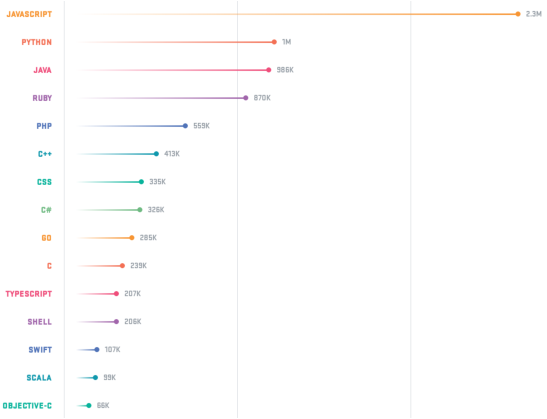
\includegraphics[scale=1.8]{github_2017.pdf}
 %\caption{As 15 linguagens mais usadas no GitHub em 2017. Fonte: \cite{githuboctoverse}}
 \caption{The 15 most used languages on GitHub in 2017. Source: \cite{githuboctoverse}}
 \label{fig:github_2017}
\end{figure}

\end{section}

\begin{section}{Parallelism in Compilation}

%O GCC é um compilador de código aberto amplamente usado tanto no meio
%acadêmico quanto na indústria. Por ser um grande projeto, o GCC contém uma
%linguagem própria para facilitar a adição de otimizações na geração de
%código, que em seguida é compilado em um único arquivo C, para (1)
%aproveitar as otimizações já implementadas no próprio compilador, e (2)
%evitar reescrever várias funcionalidades já implementadas. Infelizmente, este processo
%gera um gargalo na compilação do projeto em máquinas \textit{manycore}, pois o
%GCC não é capaz de compilar um arquivo em paralelo de maneira incremental.

%The GCC is a largely used Open Source compiler in both academic and industry
%environments. Being a large project, GCC has an additional language created to
%better express and facilitate optimizations in code generation, which is
%compiled into C++ to (1) reuse the optimizations already implemented in the
%compiler, and (2) avoid rewriting several functionalities already implemented.
%This process generates large files that must be compiled, causing a compilation
%bottleneck in the project because GCC is not capable of compiling a single file
%in parallel.

Currently, all parallelism in the compilation stage is provided either by the
GNU Make\footnote{https://www.gnu.org/software/make/}, which only provides a
per-file level granularity; or through the LTO infrastructure inside the compiler, which we
approach in Section \ref{chap:related_works}. The former, which we will label
the \textit{classical compilation method}, may bottleneck the compilation in
manycore machines if there exists some file that dominates the compilation time.
The former may also have this bottleneck if the Whole Program Analysis (WPA) stage,
which runs serially, dominates the compilation time. While parallelizing
WPA is one way of tackling this problem, we have chosen to improve the parallelization
granularity on a single file compilation of \textit{classical compilation}.


%Atualmente, todo o paralelismo na fase de compilação é provido pelo GCC de
%duas maneiras distintas: ou pelo GNU Make\footnote{https://www.gnu.org/software/make/},
%que apenas fornece uma granularidade a nível dos arquivos; ou através da estrutura do
%LTO, que será abordada na Seção \ref{chap:related_works}. Esse gargalo pode parecer uma
%característica peculiar do projeto GCC, mas discussões com a comunidade levaram
%usuários a relatar o mesmo problema em seus projetos. Tal problema pode ser
%mitigado por um compilador que seja capaz de compilar um único arquivo em paralelo
%\citep{mailgcc}. Outra possível solução seria
%partir o arquivo em arquivos menores e utilizar o esquema de
%paralelismo já existente do GNU Make, mas isto implica em uma modificação na
%estrutura do projeto, o que pode não ser o ideal.

Since today the processors' manufacturers are increasing the power of their
products through parallelism over raw sequential power, compilers that can
profit from this resource could reduce the time taken when compiling a project
or even reduce execution time on script languages that rely on Just in Time
(JIT) compilation. It means a reduction in resource usage, such as
power, time, and thus money. So far, every parallelism found internally in
optimizing compilers was a consequence of a structure created to allow more
aggressive optimizations, such as the LTO \citep{glek2010optimizing}.

%Considerando que atualmente há uma tendência para que os processadores sejam
%cada vez mais paralelos, compiladores que usufruam deste recurso poderiam
%reduzir o tempo de compilação de um projeto, ou de uma suíte de testes que
%necessita recompilação antes de sua execução, economizando recursos no caso da
%computação ser cobrada por hora. Até então, o paralelismo empregado internamente
%em compiladores otimizadores foi consequência de uma estrutura criada para
%permitir otimizações mais agressivas e custosas, como o LTO
%\citep{glek2010optimizing}.

\end{section}

\begin{section}{Research Questions}\label{sec:rq}

%Deve ser observado que nem todos os processos de um compilador podem ser
%paralelizados. Compiladores operam em etapas que podem ser fortemente
%dependentes do resultado da etapa anterior. Por exemplo, ao compilar uma
%função em C, pode ser necessário saber se alguma outra foi declarada anteriormente; ou
%então o analisador sintático pode alterar um estado do analisador léxico para
%detectar variáveis de um novo tipo. Além disto, compiladores também se apoiam em algoritmos
%em grafos, cujo paralelismo é um desafio \citep{lumsdaine2007challenges}.

We must highlight that not every process inside a compiler can be parallelized.
Compilers that operate in steps can be strongly dependent on the resource
generated by some early pass.  For instance, when compiling a function in C, it
may be necessary to know if some function was declared early; or the syntactic
analyzer may change a state in the lexical analyzer to detect variables of a
new type. Not only that, but compilers also rely on graph algorithms, in
which parallelism is not trivial \citep{lumsdaine2007challenges}.

Therefore, this work is dedicated to the following research questions:

\begin{description}
    \item[\textit{RQ1}] - What is the main point of a compiler that can be improved with parallelism?
    \item[\textit{RQ2}] - What is the performance improvement after parallelizing a compiler?
	\item[\textit{RQ3}] - When compiling in parallel is faster than compiling sequentially?
	\item[\textit{RQ4}] - How does this impact the power consumption?
\end{description}

%Sendo assim, esse trabalho concentra-se em duas questões de pesquisas:
%\begin{description}
%    \item[\textit{QP1}] - Em que pontos um compilador pode usufruir de paralelismo?
%
%    \item[\textit{QP2}] - Qual é o ganho de desempenho ao paralelizar internamente um compilador?
%\end{description}

%essas questões de pesquisa visam propor uma alternativa ao LTO com foco
%em desenvolvimento incremental, e também cobrindo os casos onde o LTO produz binários menos
%eficientes através de melhorias no paralelismo do processo clássico de compilação.
%Para validar os resultados, este trabalho inclui a implementação no GCC de algumas das
%técnicas discutidas, além da utilização de técnicas de inferência estatística para
%análises no tempo total de compilação no projeto GCC e arquivos separados.

We present answers of these questions in the hope that they may be useful to software
developers so that they be aware of how compilers may impact the development
process of their projects, as well as compiler writers about how to improve
their software using parallelism. Thus, the main contribution of this work is
to provide ways to modify an industrial-scale compiler to
compile single files in parallel.

This work is divided into the following chapters: in Chapter
\ref{chap:fundamentacao}, we present some theoretical concepts regarding
Compiler Theory, the GCC,  and Parallel Computing; to clarify some topics about this work.
Following that, Chapter \ref{chap:related_works} presents related work until
the state of art on this topic, with a brief discussion about their positive
and negative points. Then, Chapter \ref{chap:proposta} presents a general
version of the work, with an analysis of what needs to be improved,
contemplating the parallel architecture and the implementation planning, presenting
our experiments about then on Chapter \ref{cap:experiments}. Finally,
in Chapter \ref{chap:conclusions}, we present our conclusions about this work
and how this work can be improved, with future works.

This work was supported by CAPES and Google Summer of Code (GSoC). For the
latter, we present our application plans in Appendix \ref{appendex1} for the threaded
parallelism project and Appendix \ref{appendix2} for the LTO parallelism project.  

%Este trabalho está dividido nos seguintes capítulos: no Capítulo
%\ref{chap:fundamentacao}, são apresentados conceitos teóricos como parte da
%Teoria de Compiladores e Computação Paralela para que seja possível
%compreender as questões acerca do trabalho.  Em sequência, o Capítulo
%\ref{chap:related_works} contém uma apresentação dos trabalhos relacionados
%a paralelismo de compiladores até o estado da
%arte nesse tópico, além de uma breve discussão sobre seus pontos positivos
%e negativos. Por fim, o Capítulo \ref{chap:proposta} apresenta uma visão geral
%do trabalho de fato, com uma análise de tempo consumido que permitiu
%identificar quais pontos necessitam de melhorias, além da
%proposta do trabalho, que contempla a arquitetura de paralelismo e o
%planejamento de sua implementação.

\end{section}
